\section{Publicar el reporte en el portal de Power BI} 

\begin{itemize}
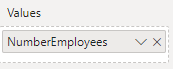
\includegraphics[scale=0.5]{./Imagenes/image032}
\item 1. En el menu principal (Home ribbon), hacer click en Publica (Publish). 
\item 2. Si pregunta por Guardar los cambios, hacer click en Guardar (Save). 

\item 3. En la ventana de Power BI Desktop, ingresar la direcciOn de correo electrónico de su cuenta Microsoft y
luego hacer click en Iniciar Sesion (Sign in). 

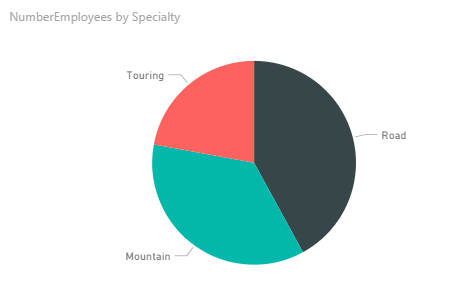
\includegraphics[scale=0.5]{./Imagenes/image033}
\item 4. En el grafico en el reporte, ajustar el tamaño del gráfico para que muestre a todo el personal de ventas. 
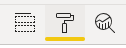
\includegraphics[scale=0.5]{./Imagenes/image018}
\item 5.El reporte sera publicado en el Portal de Power BI. Cuando la ventana muestre Satisfactorio (9Success), hacer
click en Abrir (Open) 'Ventas Adventure Works.pibx' en Power BI para ver el reporte en línea.
\\

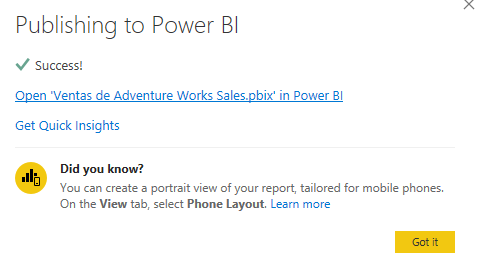
\includegraphics[scale=0.5]{./Imagenes/image034}

\item 6. Cuando el navegador se abra, hacer click en Iniciar Sesion, ingresar su correo y contraseña, Iniciar sesion, y esperar a que el reporte abra en Internet Explorer. \\

\end{itemize}